\begin{spacing}{1.5}
  \begin{tightcenter}
    \section{4. Implementación y pruebas}
    \mylinespacing
  \end{tightcenter}

  \subsection{4.1 Implementando tecnologías}

  En esta sección se explica cómo se implementó la solución propuesta. Para hacerlo fácil de reinstalar, reconfigurar y estandarizar los sistemas, así como para instalar nuevos equipos que se adquieran después de que finalice este proyecto, se creó un manual de configuración que se incluye como Anexo 1 de este documento: \textit{Instalación y configuración de los recursos informáticos de la sala de cómputo Jürgen Tischer y Clúster Bochica del Departamento de Matemáticas de la Universidad del Valle}. La implementación de las tecnologías se llevó a cabo en varias etapas, las cuales se describen en detalle en dicho anexo. Por lo tanto, se hará referencia a este múltiples veces durante la presente sección. A continuación, se presenta una descripción general de cada etapa del proceso y en qué sección del anexo 1 se puede encontrar más información.

  \subsubsection{4.1.1 Instalación en Sala de Cómputo Jürgen Tischer}

  En la sala de cómputo, como se puede visualizar en el cuaddro \ref{table:table1} del \textit{capítulo 2.1 Recursos computacionales}, existen diversos equipos de cómputo con características y capacidades variadas, por lo que algunos equipos no fueron seleccionados para formar parte del sistema distribuido debido al bajo rendimiento que pueden proveer, el cual, causaría un efecto de cuello de botella como se podrá observar más adelante en el \textit{capítulo 4.3 Pruebas de eficiencia y rendimiento}, por lo que, aunque el sistema operativo, los paquetes base y aplicaciones fueron instalados por igual en todos los equipos, solo se configuraron para trabajar en paralelos los 30 DELL PRECISION T3610 junto con los HP Z1 y Z2 para un total de 33 equipos en el sistema distribuido.

  \textbf{Configuración nodo principal}

  Para los propósitos de este proyecto se utilizó el HP Z2 como nodo principal

En primer lugar, se procedió a configurar el equipo principal, en este caso el HP Z2, debido a su capacidad de almacenamiento adicional (2 TB). Esto resultará de gran utilidad para implementar un sistema de archivos NFS que permitirá el acceso compartido a ciertos recursos por parte de todos los equipos. Tal configuración se enmarca en el diseño de una metodología que contempla la implementación de un gestor de cola de tareas con capacidades de paralelización. Por lo tanto, el uso de un equipo de mayor capacidad de almacenamiento se presenta como una medida relevante para mejorar la eficiencia del sistema distribuido.

\textbf{Configuración de NFS}

En segundo lugar, se procedió a realizar la configuración de un sistema de archivos de red (NFS) en el equipo principal, con el fin de posteriormente  habilitar el acceso de los demás equipos a los archivos compartidos. Los detalles de esta configuración se encuentran descritos en el Anexo 1, \textit{Archivos compartidos - Network File System} del presente trabajo.

\textbf{Instalación y configuración de los nodos regulares}

En tercer lugar, se realizó la instalación de los equipos en la sala de cómputo Jürgen Tischer, esto incluye instalación de Rocky Linux 9, configuración de repositorios y manejadores de paquetes, configuración para el acceso de NFS. Se siguieron los procedimientos estándar para la instalación de equipos de cómputo descritos en el Anexo 1, Sección: \textit{Instalación y configuración inicial del sistema}, asegurándose de que los equipos estuvieran conectados correctamente y de que estuvieran configurados para funcionar en la red del departamento de matemáticas.

\textbf{Instalación y configuración de herramientas de Wolfram}

La cuarta etapa del proceso involucró la instalación del manejador de licencias de Mathematica MathLM, este se instaló en el nodo principal para proporcionar las licencias de Mathematica de una forma centralizada. Posteriormente se realizó la instalación y configuración de Mathematica y gridMathematica en los demás nodos del sistema distribuido. La instalación de MathLM, Mathematica y gridMathematica se describe en detalle en el Anexo 1, Sección: \textit{Mathematica, gridMathematica y MathLM.}

\subsubsection{Instalación en Clúster Bochica}

En el Clúster Bochica, como se puede visualizar en el cuadro \ref{table:table1} del capítulo 2.1 \textit{Recursos computacionales}, existen 2 tipos de servidores computacionales con distintas características y capacidades, 4 unidades de cada tipo de equipo, en este caso se tomaron todas las 8 unidades para hacer parte del sistema distribuido. También se escogió uno de los HP DL360E como nodo principal.

\textbf{Configuración de Switch en el Clúster}

El Clúster posee un Switch de Ethernet de alta velocidad que permite a los nodos conectarse entre sí, también con el resto de la red universitaria y a internet. Este switch había sido configurado con anterioridad para que solo unos nodos en particular pudiesen acceder a internet, por lo que se reconfiguró para que se pudieran conectar entre ellos y con internet, que es requerido para la instalación de paquetes de los repositorios. Los detalles se encuentran en el Anexo 1, Sección: \textit{Clúster / Configuración Switch}.

\textbf{Instalación y configuración inicial del sistema}

Posterior a la configuración del Switch, se procedió a la instalación y configuración del sistema operativo de los nodos del clúster. Aunque la instalación es muy similar a la de los computadores en la Sala Jürgen Tischer, se toma una base dintinta que no requiere interfaz gráfica y no se realiza la instalación de aplicaciones gráficas, en cambio se instalan otras librerías que son necesarias para su correcto funcionamiento. La instalación de los nodos del clúster se describe en detalle en el Anexo 1, Sección: \textit{Clúster / Instalación y configuración inicial del sistema.}

\textbf{Configuración de NFS}

Posterior a la instalación de los sistemas operativos de cada uno de los servidores, se procedió a configurar uno de los HP DL360E como nodo principal. Este equipo fue configurado para funcionar como nodo principal del Clúster Bochica, por lo que se configurará para que comparta la carpeta de /home con los demás nodos, esto se hace para que los trabajos de slurm, ejecutados desde Jupyterhub por los distintos usuarios, cada uno en su directorio personal, puedan acceder a los archivos desde todos los nodos desde los que sean ejecutados. Lo cual se describe en detalle en el Anexo 1, Sección: \textit{Clúster / Configuración de NFS.}

\textbf{Configuración de conda y Jupyterhub con componentes adicionales}

En la siguiente etapa, se realizó la instalación de Conda. Conda es un sistema de gestión de paquetes que se utiliza para instalar y administrar paquetes y dependencias de software principalmente relacionadas con Python. La instalación de conda se describe en detalle en el Anexo 1, Sección: \textit{Clúster / Instalación de Conda.}

Mediante el uso de Conda se procedió a la configuración de 3 ambientes, Un ambiente completo con los paquetes de Anaconda, que representa una instalación de Python bastante completa a la que se le agregó mpi4py para el manejo del clúster y los paquetes necesarios para la ejecución de Jupyterhub, este ambiente es el principal del clúster. También se configuró un segundo ambiente con SageMath y un tercer ambiente con R. Los detalles de la instalación de estos ambientes y la demás configuración de Jupyterhub puede encontrarse en el Anexo 1, Sección: \textit{Configuración Jupyterhub}

\textbf{Instalación y configuración de SLURM}

Por último, se llevó a cabo la instalación y configuración de Slurm. Slurm es un sistema de gestión de trabajos que permite a múltiples usuarios lanzar un trabajo para que se ejecute cuando los recursos del sistema se encuentren disponibles. La instalación y configuración de Slurm se describe en detalle en el Anexo 1, Sección: \textit{Slurm}.

Cabe recalcar que el Anexo 1 proporciona detalles completos sobre cada una de estas etapas, así como información adicional sobre la configuración y el funcionamiento del sistema distribuido tanto en la Sala Jürgen Tischer como en el Clúster Bochica. Además de destacar que la guía se elaboró cuidadosamente para garantizar que el sistema puediera ser fácilmente recreado a partir de recursos no necesariamente idénticos.

\subsubsection{4.1.3 Comunicación del servicio funcionando}

Finalmente se procedió a dar la comunicación al departamento de matemáticas sobre la implementación de las tecnologías y herramientas en la Sala de Cómputo Jürgen Tischer y el Clúster Bochica. Se les informó sobre las ventajas y beneficios que estas herramientas ofrecen para la realización de tareas de cómputo distribuido y se les brindó una guía de uso y acceso. También se realizó una charla abierta, principalmente dirigida a los profesores del departamento y estudiantes de posgrado que estuvieran interesados en el servicio.

  \subsection{4.2 Pruebas de control}

  En el proceso de verificar el correcto funcionamiento de los computadores y las integraciones, se emplean diversas herramientas, como las presentadas a continuación.

  \subsubsection {4.2.1 Comprobar conectividad básica con pdsh}

  El comando \code{alias} se configuró para verificar el estado de los equipos
  en
  el clúster. Este comando permite lanzar un comando de manera más sencilla,
  por
  ejemplo, \code{pdsh xeon "hostname"}, que devuelve el nombre de
  todos los
  equipos encendidos y conectados correctamente por ssh. Además, si se utiliza
  el
  argumento \code{uptime} en vez de \code{hostname}, se puede obtener más
  información sobre el estado de cada nodo.

  El resultado se ve de esta forma :

  \definecolor{codebackground}{RGB}{240,240,240}
  % Color de fondo del código
  \definecolor{codecomment}{RGB}{100,100,100}
  % Color de los comentarios
  \definecolor{codekeyword}{RGB}{0,0,255}
  % Color de las palabras clave
  \definecolor{codestring}{RGB}{163,21,21}
  % Color de las cadenas de texto

  \lstset{
    backgroundcolor=\color{codebackground},
    commentstyle=\color{codecomment},
    keywordstyle=\color{codekeyword},
    stringstyle=\color{codestring},
    basicstyle=\footnotesize\ttfamily,
    breakatwhitespace=false,
    breaklines=true,
    captionpos=b,
    frame=single,
    numberstyle=\tiny\color{codecomment},
    showspaces=false,
    showstringspaces=false,
    showtabs=false,
    tabsize=2,
    rulecolor=\color{codebackground}
  }
  \begin{lstlisting}[language=C]
      $ xeon "hostname"
      C4: C4
      E3: E3
      A2: A2
      ...
      B5: B5
  \end{lstlisting}

  \subsubsection {4.2.2 Comprobar funcionamiento en Mathematica}

  En Mathematica es fácil comprobar que la configuración paralela funciona
  correctamente. Para hacerlo, seleccione una configuración sencilla que
  incluya
  todos los nodos que desea utilizar. En nuestro caso, configuramos Lightweight
  Grid en las opciones de configuración paralela del kernel, con un kernel
  disponible para cada nodo. También es necesario desactivar
  \textit{RemoteKernel
    Objects}, que es un configurador automático que, por defecto, solo usa los
  kernels locales e ignora toda la configuración que se le coloca. Los kernels
  configurados se muestran en la Figura \ref{fig:etiqueta1}.  \newline  \newline

  \begin{figure}[h]
    \centering
    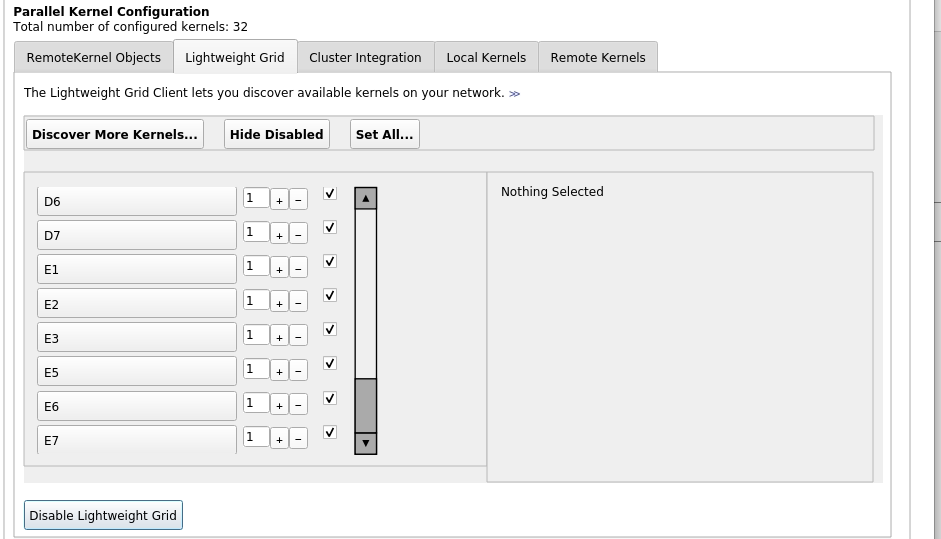
\includegraphics[width=0.9\textwidth]{mat.png}
    \caption{Configuración paralela en Mathematica}
    \label{fig:etiqueta1}
  \end{figure}

  Una vez que se haya completado esta configuración, podrás abrir un nuevo
  cuaderno (notebook) y escribir la siguiente instrucción: \code{LaunchKernels[
      ]}. De esta manera, la aplicación tratará de conectarse con los kernels
  configurados en cada nodo, tal como se muestra en la Figura
  \ref{fig:etiqueta2}

  \begin{figure}[h]
    \centering
    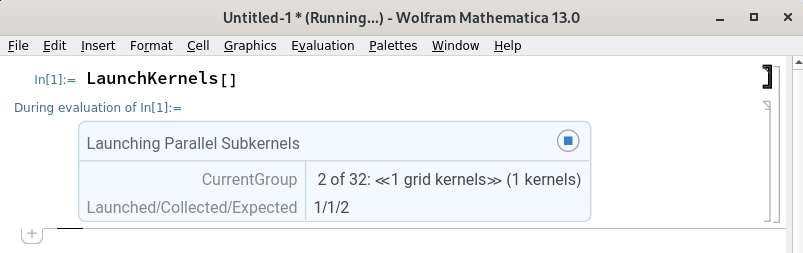
\includegraphics[width=0.9\textwidth]{mat1.png}
    \caption{Conexión de kernels y nodos}
    \label{fig:etiqueta2}
  \end{figure}

  En caso de que todo salga bien, se muestra una lista con todos los kernels
  iniciados, como se indica en la Figura \ref{fig:etiqueta3}

  \begin{figure}[h]
    \centering
    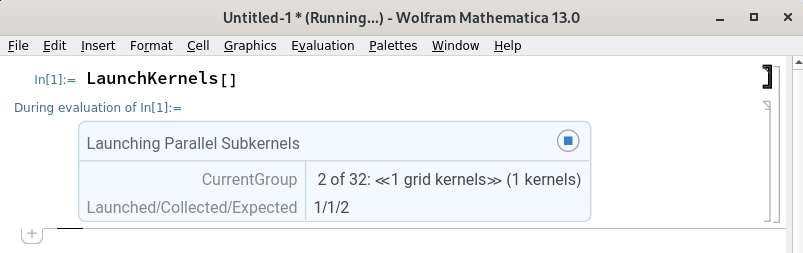
\includegraphics[width=0.9\textwidth]{mat4.png}
    \caption{Kenerls iniciados}
    \label{fig:etiqueta3}
  \end{figure}

  Si hay un error, Mathematica lo señalará. Normalmente el error incluirá
  información sobre el nodo que presenta problemas, así como una breve
  descripción del problema y posibles soluciones a aplicar, en la Figura
  \ref{fig:etiqueta4} se puede observa un error en Mathematica.

  \begin{figure}[h]
    \centering
    
\includegraphics[width=0.9\textwidth]{mat3.png}
    \caption{Información de error}
    \label{fig:etiqueta4}
  \end{figure}

  \subsubsection {4.2.3 Comprobar funcionamiento en Slurm}

  En Slurm, hay varios comandos básicos que nos permiten ver información sobre
  el
  estado de los nodos configurados.

  \begin{itemize}
    \item \textbf{sinfo}: Muestra el estado de los nodos. Es la primera
          herramienta que se debe utilizar para visualizar si hay algún
          problema de
          comunicación con los nodos.
    \item \textbf{srun}: Agrega una tarea a la cola de manera activa.
    \item \textbf{squeue}: Muestra la lista de tareas en cola, tanto pendientes
          como en ejecución.
    \item \textbf{scancel}: Cancela una tarea que se encuentra en la cola.
    \item \textbf{scontrol}: Se utiliza principalmente para cambiar el estado
          de los nodos.
  \end{itemize}

  Es posible probar rápidamente el funcionamiento de los nodos con \code{srun},
  de manera similar a como se utilizaba \code{pdsh}. En este caso, el comando
  utilizado es \code{srun -N10 hostname}. Esto solicitará a 10 nodos
  disponibles
  que ejecuten el comando \code{hostname}, devolviendo sus nombres. Si se
  utiliza
  el número total de nodos y todos devuelven su nombre, entonces la
  comunicación
  básica funciona. Sin embargo, solo esta prueba no es suficiente para
  determinar
  un problema de sincronización, ya que puede haber un problema en la
  comunicación del número de nodos en la tarea, donde cada nodo cree que es el
  único que ejecuta la tarea y no se da cuenta de que hay otros.

  \textbf{Helloworld Paralelo con C y C++}

  Para verificar la comunicación completa, se utilizó el programa de ``hola
  mundo''
  en paralelo con MPI, escrito en C. Esto se basa en el tutorial de
  mpitutorial.com \cite{HelloC}:

  \definecolor{codebackground}{RGB}{240,240,240}
  % Color de fondo del código
  \definecolor{codecomment}{RGB}{100,100,100}
  % Color de los comentarios
  \definecolor{codekeyword}{RGB}{0,0,255}
  % Color de las palabras clave
  \definecolor{codestring}{RGB}{163,21,21}
  % Color de las cadenas de texto

  \lstset{
    backgroundcolor=\color{codebackground},
    commentstyle=\color{codecomment},
    keywordstyle=\color{codekeyword},
    stringstyle=\color{codestring},
    basicstyle=\footnotesize\ttfamily,
    breakatwhitespace=false,
    breaklines=true,
    captionpos=b,
    frame=single,
    numberstyle=\tiny\color{codecomment},
    showspaces=false,
    showstringspaces=false,
    showtabs=false,
    tabsize=2,
    rulecolor=\color{codebackground}
  }

  \begin{lstlisting}[language=C]
    #include <stdio.h>
    #include <unistd.h>
    #include <mpi.h>
    
    int main(int argc, char** argv)
    {
      // Init the MPI environment
      MPI_Init(NULL, NULL);
      // Get the number of processes
      int world_size;
      MPI_Comm_size(MPI_COMM_WORLD, &world_size);
      // Get the rank of the process
      int world_rank;
      MPI_Comm_rank(MPI_COMM_WORLD, &world_rank);
      // Get the name of the processor
      char processor_name[MPI_MAX_PROCESSOR_NAME];
      int name_len;
      MPI_Get_processor_name(processor_name, &name_len);
      // Print a hello world message
      printf("Hello, World! from node %s, rank %d out of %d processors\n",
             processor_name, world_rank + 1, world_size);
      // Finalize the MPI environment
      MPI_Finalize();
    }
    \end{lstlisting}

  Para compilar este código es necesario contar con mpicc. Para hacerlo, se
  debe utilizar el siguiente comando: \code{mpicc c-mpi-hello.c -o
    c-mpi-hello}.

  Luego, el archivo debe ser accesible desde todas las máquinas en la misma
  ubicación. Para lograr esto, se utilizó un NFS, tal como se indica en la guía
  adjunta en el apartado NFS.

  Para ejecutar el código, se debe utilizar el comando \code{srun -N10
    /nfs/c-mpi-hello}.Esto asignará 10 nodos, cada uno con un hilo de proceso. El resultado tiene el siguiente formato :

    \begin{lstlisting}[language=C]
      $ srun -N4 c-mpi-hello
      Hello, World! from node bochica2, rank 2 out of 4 processors
      Hello, World! from node bochica3, rank 3 out of 4 processors
      Hello, World! from node bochica1, rank 1 out of 4     processors
      Hello, World! from node bochica4, rank 4 out of 4 processors
    \end{lstlisting}

  \textbf{Helloworld Paralelo con Python}

  Se puede lograr lo mismo utilizando Python. Se recomienda preparar un
  entorno utilizando conda o mamba en el NFS para que esté disponible para
  todos
  los nodos involucrados. Además, el entorno debe contener el paquete
  \code{mpi4py}. En nuestro caso, utilizamos la implementación de \code{mpich}.
  El entorno fue creado con el comando \code{conda create -p /nfs/anaconda}
    \code{anaconda mpi4py mpich}.

    En el siguiente código se muestra un programa en Python utilizando mpi4py para imprimir Hello World

    \begin{lstlisting}[language=python]
      # py-mpi-hello.py
      """
      Parallel Hello World
      """

      from mpi4py import MPI
      import sys
      import getpass

      size = MPI.COMM_WORLD.Get_size()
      rank = MPI.COMM_WORLD.Get_rank()
      name = MPI.Get_processor_name()
      user = getpass.getuser()

      sys.stdout.write(
      "%s: Hello, World! I am process %d of %d on %s.\n"
      % (user, rank+1, size, name))

    \end{lstlisting}
      
    Para activar el entorno de conda durante la ejecución de cada nodo, es más conveniente utilizar un archivo de sbatch que directamente con srun como se muestra a continuación:

    \begin{lstlisting}[language=python]
      # py-mpi-hello.sbatch
      #!/bin/sh
      #SBATCH -o /nfs/sbatch-examples/helloworld/py-mpi-hello.out
      #SBATCH --nodes=4
      #SBATCH --ntasks-per-node=1

      # Load conda commands from local installation
      source /opt/conda/etc/profile.d/conda.sh

      # Activate shared conda on nfs
      conda activate /nfs/conda

      # Run mpi example
      srun python /nfs/sbatch-examples/helloworld/py-mpi-hello.py
    \end{lstlisting}

    Utilizamos \code{sbatch py-mpi-hello.sbatch} para ejecutar la prueba y verificar su funcionamiento. El resultado debe ser como se muestra a continuación:

      \begin{lstlisting}[language=python]
      estudiante: Hello, World! I am process 2 of 4 on bochica2.
      estudiante: Hello, World! I am process 3 of 4 on bochica3.
      estudiante: Hello, World! I am process 4 of 4 on bochica4.
      estudiante: Hello, World! I am process 1 of 4 on bochica1. 
      \end{lstlisting}
      
  \subsection{4.3 Pruebas de eficiencia}  \label{chap:4.3}

      Se llevaron a cabo dos pruebas para evaluar el rendimiento de los sistemas implementados. La primera prueba se realizó utilizando gridMathematica para resolver un sistema polinomial de ecuaciones y midió el rendimiento al variar el tamaño de un problema y la cantidad de nodos utilizados para resolverlo. La segunda prueba utilizó Slurm para resolver un sistema denso de ecuaciones lineales mientras variaba la cantidad de nodos utilizados para resolver dicho problema.   

      \subsubsection{4.3.1 Prueba de gridMathematica}

      Para probar el rendimiento en singular, multi-proceso y multi-máquina utilizamos el código de uno de los proyectos que se beneficiaron con la implementación de esta tesis (ver Capítulo 5, Influencia en proyectos destacados, para más detalles).

      De este código nos interesaremos por una parte en particular en donde existe una variable de puntos que afectan a un problema lineal, el cual resulta óptimo para probar el rendimiento de los sistemas.

      Preprint del proyecto mencionado y código de GitHub a utilizar. \cite{preprint} \cite{git}

      Para las pruebas utilizamos diferentes escenarios, un DELL PRECISION T3610 equipado con Intel Xeon E5-1620 v2 @ 3.9GHz (4 núcleos físicos, 8 hilos de ejecución), lo comparamos con un HP Z1 equipado con un Intel i9-10900 @ 5.2 GHz para ver la diferencia de velocidad al escalar verticalmente una máquina y luego con el mismo Intel Xeon pero con 10 de esos.

      Las pruebas realizadas tenían como objetivo observar 3 puntos clave:

      \begin{itemize}
            \item Visualizar la diferencia en la ejecución del mismo problema al asignar la cantidad de núcleos físicos, en comparación con la asignación de la cantidad total de hilos de ejecución en una máquina.
            \item Mostrar la variación de complejidad en el problema según se varía su tamaño.
            \item Evidenciar la optimización de la ejecución al distribuir el problema en el sistema.
      \end{itemize}

      \subsubsection{4.3.2 Resultados Mathematica}

      \textbf{Nota:} En los resultados mostrados solo se considera el tiempo de ejecución del cálculo realizado, no se toma en cuenta el tiempo que tarda en conectar los nodos ni en preparar las variables. Es por eso que cabe resaltar que el tiempo de conexión de los nodos, en gridMathematica para 30 nodos, puede tardar más de 4 minutos.

      En las gráficas los nombres Xeon e i9 hacen referencia a este tipo de equipos utilizados: 

      \begin{itemize}
            \item Xeon: DELL PRECISION T3610, Xeon E5-1620 v2 @ 3.9GHz 
            \item i9: HP Z1, i9-10900 @ 5.2 GHz
      \end{itemize}

      Según los datos de la tabla 1 del anexo 2, podemos ver la gráfica \ref{fig:etiquetaa}. Se observa que asignar una cantidad alta de procesos a una tarea no necesariamente mejora el rendimiento. De hecho, si la cantidad de hilos supera la cantidad de núcleos físicos, esto puede empeorar el resultado. Por lo tanto, es importante considerar el número de núcleos físicos cuando se asignan procesos a una tarea para garantizar un rendimiento óptimo.

      Así mismo, el uso de más procesos puede aumentar significativamente el consumo de memoria RAM, lo que a su vez puede afectar el rendimiento general del sistema. Es recomendable evaluar cuidadosamente el número de procesos que se asignan a una tarea y tomar medidas para optimizar el uso de la memoria RAM. Por ejemplo, se puede configurar la memoria virtual. Además, es importante tener en cuenta que, aunque el uso de múltiples procesos puede aumentar el rendimiento en algunos casos, también puede aumentar la complejidad del sistema y dificultar su mantenimiento y depuración.\newpage

      \begin{figure}[h]
            \centering
            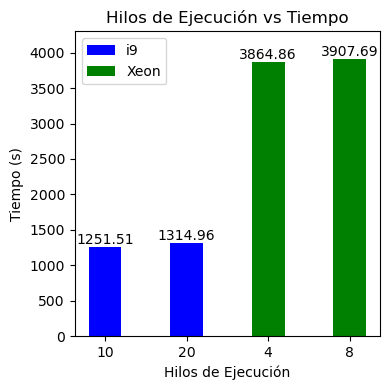
\includegraphics[width=0.5\textwidth]{tab1.png}
            \caption{Hilos de Ejecución vs Tiempo}
            \label{fig:etiquetaa}
          \end{figure}

          En la gráfica \ref{fig:etiquetab}, que se obtiene de los datos de la tabla 2 del anexo 2, se separan los datos según la configuración del sistema. Se utilizan 5 configuraciones en total, y se establece la configuración de referencia como 1 nodo Xeon.

          La gráfica muestra que, al escalar verticalmente (es decir, al ejecutar el problema en un solo nodo más potente), el tiempo de ejecución puede reducirse drásticamente. Sin embargo, al escalar horizontalmente (es decir, añadiendo más nodos a la ejecución), se pueden obtener resultados que no son fácilmente alcanzables al escalar verticalmente. De hecho, al utilizar 30 nodos Xeon, se puede llegar a tener un tiempo casi 10 veces menor.
          
          Otra cosa que se puede evidenciar en la gráfica es que, según se aumenta el número de puntos, el problema escala con una tendencia lineal, como se esperaba en un principio. Además, la linealidad se mantiene constante a medida que se agregan más puntos, lo que sugiere que el problema no se vuelve más complejo a medida que se incrementa el número de puntos. En general, la gráfica proporciona una idea clara de cómo se comporta el problema a medida que se varía el número de puntos, lo que permite una mejor comprensión del mismo en términos de complejidad y escalabilidad. \newpage

      \begin{figure}[h]
            \centering
            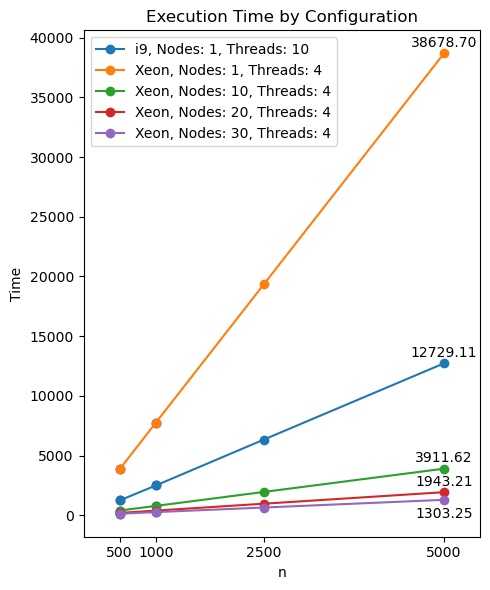
\includegraphics[width=0.5\textwidth]{tab2.png}
            \caption{Tiempo de ejecución por configuración}
            \label{fig:etiquetab}
      \end{figure} 

      La gráfica \ref{fig:etiquetac} muestra los datos de la tabla 3 del Anexo 2,
      considerando solo \textit{n = 5000}Se midió el tiempo de ejecución con
      diferentes configuraciones de Xeon, y se comparó la mejora temporal
      obtenida al utilizar 10, 20 y 30 nodos, tomando el tiempo de 1 solo nodo
      como tiempo de referencia.
      
      Los resultados obtenidos arrojaron información relevante sobre la
      eficiencia de los diferentes nodos en relación con el tiempo de ejecución,
      ya que se obtuvo una mejora en el rendimiento de aproximadamente el 98.9\%,
      con respecto al valor de referencia, por cada nodo agregado. lo que
      demuestra una estabilidad en la distribución del problema que utiliza el
      software de gridMathematica, lo cual resulta importante en la
      escalabilidad para este tipo de problemas a gran escala.

      \begin{figure}[h]
            \centering
            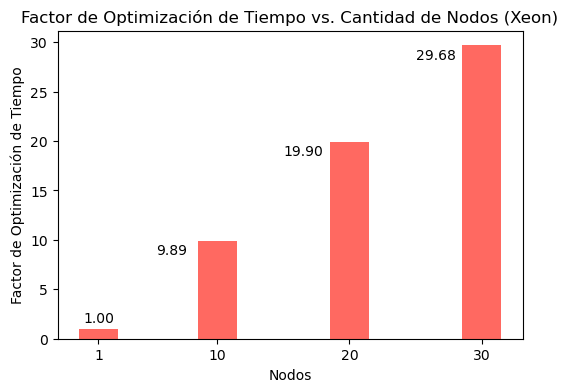
\includegraphics[width=0.5\textwidth]{tab3.png}
            \caption{Factor de Optimización de Tiempo vs. Cantidad de Nodos (Xeon)}
            \label{fig:etiquetac}
      \end{figure}

      En términos generales, es importante tener en cuenta que cuando se trata de problemas pequeños, puede ser más eficiente resolverlos en un solo nodo, ya que el tiempo de conexión entre nodos puede ser significativo. Sin embargo, cuando se trata de un problema a gran escala, la distribución se convierte en un factor clave para su resolución. En estos casos, el uso de software como gridMathematica puede ser de gran ayuda para distribuir el problema y obtener beneficios netos en la resolución. Además, es importante destacar que esta distribución no solo permite una resolución más rápida, sino que también puede permitir una mejor utilización de los recursos disponibles.

\subsubsection{4.3.3 Slurm - The Linpack Benchmark para sistemas distribuidos}

El benchmark Linpack es una prueba de rendimiento computacional que mide la capacidad de cálculo y eficiencia de un sistema informático en términos de velocidad y procesamiento numérico. Fue diseñado por Jack Dongarra en los años 70 en el Laboratorio Nacional de Oak Ridge, y se ha convertido en un estándar en el campo de la supercomputación y el rendimiento de los sistemas informáticos. \cite{linpack},  \cite{faq-linpack}

Para nuestra prueba utilizaremos HPL, una implementación portable del Linpack Benchmark para sistemas con memoria distribuida. HPL es un paquete de software que resuelve un sistema lineal (aleatorio) denso en aritmética de doble precisión (64 bits) en equipos con memoria distribuida.\cite{hpl-linpack}

Con esta prueba, es posible evaluar el rendimiento y la capacidad de procesamiento de diferentes configuraciones computacionales y compararlos. En este proyecto, se utilizó Slurm para ejecutar la prueba en sistemas distribuidos. Se realizaron pruebas con diferentes cantidades de nodos, lo que permitió medir el rendimiento en distintos escenarios.

Para configurar la prueba de manera adecuada, se utilizó una herramienta web que genera una recomendación de configuración según la cantidad de nodos, la cantidad de tareas por nodo y la cantidad de memoria.\cite{tune-hpl-dat-file}

Con esta herramienta se configuró un archivo base que se cambiaría según la cantidad de nodos a utilizar. El archivo HPL.dat base que se tomó para las pruebas es tal que:

\begin{lstlisting}[language=bash]
      HPLinpack benchmark input file
Innovative Computing Laboratory, University of Tennessee
HPL.out      output file name (if any)
6            device out (6=stdout,7=stderr,file)
1            # of problems sizes (N)
34176         Ns
1            # of NBs
192           NBs
0            PMAP process mapping (0=Row-,1=Column-major)
1            # of process grids (P x Q)
1            Ps
1            Qs
16.0         threshold
1            # of panel fact
2            PFACTs (0=left, 1=Crout, 2=Right)
1            # of recursive stopping criterium
4            NBMINs (>= 1)
1            # of panels in recursion
2            NDIVs
1            # of recursive panel fact.
1            RFACTs (0=left, 1=Crout, 2=Right)
1            # of broadcast
1            BCASTs (0=1rg,1=1rM,2=2rg,3=2rM,4=Lng,5=LnM)
1            # of lookahead depth
1            DEPTHs (>=0)
2            SWAP (0=bin-exch,1=long,2=mix)
64           swapping threshold
0            L1 in (0=transposed,1=no-transposed) form
0            U  in (0=transposed,1=no-transposed) form
1            Equilibration (0=no,1=yes)
8            memory alignment in double (> 0)
##### This line (no. 32) is ignored (it serves as a separator). ######
0                               Number of additional problem sizes for PTRANS
1200 10000 30000                values of N
0                               number of additional blocking sizes for PTRANS
40 9 8 13 13 20 16 32 64        values of NB

\end{lstlisting}

Para todas las pruebas, se mantuvo constante el tamaño del problema, representado por el valor de Ns, que en este caso fue de 34176. Para el valor de P y Q, que determinan cómo se distribuirá el problema, se realizaron dos variaciones. La primera, llamada P y Q recomendados, fue la recomendada por la herramienta web. La segunda, llamada Normal, tiene P igual al número de procesos por nodo y Q igual al número de nodos, es decir, en este caso, P es igual a 4, ya que utilizaremos la cantidad de procesos por nodo igual al número de núcleos físicos por nodo.

\subsubsection{4.3.4 Resultados Slurm - The Linpack Benchmark para sistemas distribuidos}

Durante la realización de esta tesis, se presentaron circunstancias imprevistas que afectaron el desarrollo de las pruebas de rendimiento en el entorno del clúster Bochica. Se detectaron problemas de mantenimiento en dicho entorno que comprometían su disponibilidad y estabilidad, poniendo en riesgo la precisión y confiabilidad de los resultados obtenidos.

En vista de esta situación, se tomó la decisión de replicar el entorno de Slurm utilizando los computadores DELL PRECISION T3610 con Xeon E5-1620 v2 de la sala, mismos computadores de la prueba de Mathematica, en donde se procedió a ejecutar las pruebas de rendimiento. Aunque esta medida no estaba contemplada originalmente en el plan de investigación, se consideró como la mejor alternativa disponible para asegurar la integridad de las pruebas y la obtención de resultados fiables.

Cabe destacar que se tomaron todas las medidas necesarias para garantizar que el entorno secundario contara con una configuración similar al entorno Bochica, asimismo se minimizaron las diferencias de entorno a fin de mantener la consistencia en las pruebas realizadas.

Durante la ejecución de las pruebas, se identificó la existencia de un nodo con deficiencias en su capacidad de comunicación con el resto del sistema, lo cual resultaba en una disminución general en la velocidad de las pruebas. Ante la presencia de este nodo problemático, se llevó a cabo la ejecución de las pruebas tanto con la configuración estándar como con la configuración recomendada, asegurando la exclusión de dicho nodo en la participación. Con fines investigativos, se introdujo una nueva configuración estándar en la cual se garantizaba la presencia de este nodo problemático, permitiendo así comparar cómo su influencia afectaba los resultados obtenidos.

Los resultados de las pruebas se encuentran documentados en las tablas 4, 5 y 6 del Anexo 2. En las gráficas \ref{f:Gflops} y \ref{f:Tiempo}, se presenta una representación visual de los Gflops (mil millones de operaciones de punto flotante por segundo) y el tiempo requerido por cada prueba en relación a la cantidad de nodos utilizados, siguiendo las configuraciones previamente mencionadas.

En líneas generales, estos datos ofrecen una perspectiva sobre la variación del rendimiento del sistema en relación con el número de nodos y tareas por nodo. En términos generales, se observa una mejora en el rendimiento a medida que se incrementa la cantidad de nodos y tareas, aunque esta mejora no es de naturaleza lineal debido a los desafíos asociados con la comunicación y la sobrecarga inherentes a la coordinación entre los nodos.

\begin{figure}
 \centering
  \subfloat[Gflops vs Nodos]{
   \label{f:Gflops}
    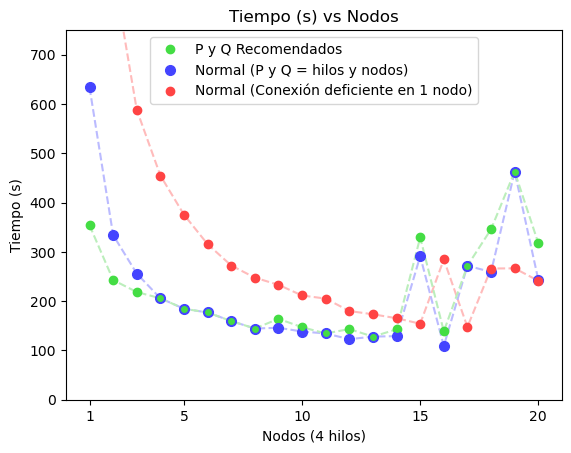
\includegraphics[width=0.5\textwidth]{1.png}}
  \subfloat[Tiempo vs Nodos]{
   \label{f:Tiempo}
    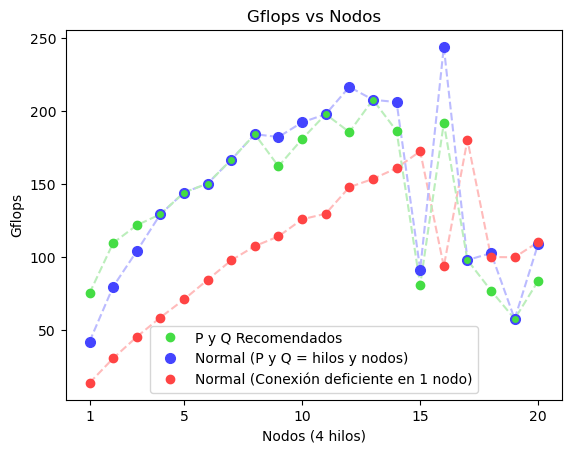
\includegraphics[width=0.5\textwidth]{2.png}}
 \caption{Comportamientos de nodos}
 \label{f:nodos}
\end{figure}

Sin embargo esta tendencia ascendente en el rendimiento a medida que se incrementa el número de nodos, alcanza un punto donde la adición de nodos adicionales no parece tener el efecto deseado, conduciendo a resultados generalmente inferiores. Es relevante destacar que estos resultados se mantienen consistentes a lo largo de múltiples iteraciones de las pruebas, lo que indica que la tendencia observada en la gráfica es persistente con ligeras variaciones para cada prueba en particular. Esta observación sugiere que, posiblemente debido al tamaño reducido del problema, incorporación de nodos adicionales introduce dificultades de comunicación en lugar de brindar un rendimiento mejorado de manera ilimitada. Esta circunstancia podría atribuirse a la distribución del problema entre los nodos involucrado, es decir, cuando la cantidad de nodos destinados a abordar el problema excede a los óptimos para la resolución de un problema, los resultados pueden mostrar una tendencia imprevista.

Además, es pertinente resaltar otra observación de relevancia en relación al resultado que involucra un nodo con una conexión deficiente en la prueba. A pesar de haber utilizado una configuración normal, los resultados obtenidos son significativamente inferiores en comparación con la configuración estándar. En general, se concluye que los resultados podrían haber sido mejores si no se hubiera empleado dicho nodo en su totalidad.

Por otro lado, la adopción de los valores recomendados de P y Q, si bien arrojó resultados apreciables, no siempre resultó ser la opción más favorable. Por lo tanto, no es posible concluir de manera definitiva cuál de las dos configuraciones es más efectiva. No obstante, se observa que la configuración denominada como "normal" exhibe una mayor estabilidad en términos generales.

  \subsection{4.4 Automatización - Facilitar el uso}   \label{chap:4.4}

  \subsubsection{4.4.1 Scripts}

  En el desarrollo de este proyecto, se llevaron a cabo diversos scripts de
  automatización que permiten realizar tareas de mantenimiento y configuración
  de
  manera más eficiente y sistemática. Estos scripts han sido diseñados para
  optimizar procesos específicos dentro del proyecto y su implementación ha
  permitido reducir el tiempo de ejecución de tareas repetitivas y mejorar la
  calidad del trabajo.

  Estas son las funciones principales de los scripts de automatización:

  \begin{itemize}
    \item Encendido y apagado de computadores.
    \item Verificación del estado de los computadores y servicios.
    \item Actualización de software.
    \item Instalación de paquetes de software.
    \item Configuración completa de un nuevo equipo recién instalado o de
          un equipo antiguo formateado.
  \end{itemize}

  Esto permitirá minimizar las tareas comunes y de mantenimiento requeridas
  con menor esfuerzo. Además, estos scripts son altamente escalables y pueden
  ser
  adaptados para su uso en proyectos futuros, lo que representa una inversión a
  largo plazo en la mejora de la eficiencia y la calidad del trabajo.\cite{github}

  \subsection{4.5 Problemas encontrados}
  En el desarrollo de este proyecto, se presentaron problemas tanto previstos
  como inesperados, los cuales serán mencionados a continuación.

  \subsubsection{4.5.1 Problemas esperados}

  \begin{enumerate}
    \item \textbf{Heterogeneidad de los recursos computacionales:} El clúster
          Bochica y la sala de computación Jürgen Tischer contienen una
          variedad de
          recursos computacionales, incluyendo diferentes tipos de
          computadoras, sistemas
          operativos y versiones de software. Esto puede dificultar la
          optimización del
          sistema distribuido diseñado y requerir una mayor planificación y
          flexibilidad
          en el diseño y la implementación.
    \item \textbf{Antigüedad de los computadores:} Algunos de los computadores
          en el clúster Bochica y la sala de computación Jürgen Tischer son
          antiguos y
          pueden tener un impacto en la eficiencia y la capacidad de ejecutar
          tareas de
          investigación de manera óptima.
    \item \textbf{Dificultades en la adaptación a las nuevas herramientas:} La
          implementación de nuevas herramientas y tecnologías puede requerir un
          período
          de adaptación y aprendizaje para los usuarios, lo que puede retrasar
          los
          procesos de investigación y enseñanza. Además, pueden surgir
          problemas técnicos
          durante la instalación y configuración de las herramientas, lo que
          puede
          interferir en la eficiencia y productividad.
  \end{enumerate}

  \subsubsection{4.5.2 Problemas no esperados}

  \textbf{Problemas con el software}

  \begin{itemize}
    \item Problemas de licencias: Parte del software utilizado era
          propietario y resultó problematico el correcto uso de estas
          licencias,
          especialmente el software de Wolfram Mathematica.
  \end{itemize}

  \textbf{Problemas con el hardward}

  \begin{itemize}
    \item Cables mal acomodados: Los cables del clúster estaban mal
          acomodados, lo que generaba una dificultad para conocer las
          diferentes
          interconexiones entre los recursos.
    \item Cables faltantes: Se encontró que se requería un cable serial
          para la adecuada configuración de un switch que permite la
          interconexión entre
          los equipos del clúster.
    \item Permisos olvidados: Varios equipos del clúster debido a su
          desuso, se habían perdido las credenciales para utilizarlos de la
          manera
          adecuada
    \item Partes que requerían mantenimiento: Algunas partes del hardware
          requerían mantenimiento para su óptimo funcionamiento, pero esto no
          se había
          realizado.
    \item Desconocimiento de las limitaciones del hardware: Al principio no
          se conocían las limitaciones del hardware, lo que dificultaba su
          correcto uso y
          aprovechamiento.
    \item Hardware mal acomodado: El hardware estaba mal acomodado, lo que
          generaba problemas en la conexión y en el acceso a los recursos
          computacionales.
  \end{itemize}

  \textbf{Problemas con la Implementación del Sistema Distribuido}

  \begin{itemize}
    \item Falta de documentación clara para la implementación: La
          documentación para la implementación del sistema distribuido no era
          clara, lo
          que dificultaba su correcta implementación.
    \item Dificultades en la integración de los diferentes componentes del
          sistema: Se encontraron dificultades en la integración de los
          diferentes
          componentes del sistema distribuido, lo que limitaba su correcto
          funcionamiento.
    \item Limitaciones en la capacidad de paralelización: Se encontraron
          limitaciones en la capacidad de paralelización del sistema
          distribuido, lo que
          disminuía su eficiencia y efectividad.
  \end{itemize}

  \textbf{Problemas con las Herramientas Instaladas}

  \begin{itemize}
    \item Falta de compatibilidad con otras aplicaciones: Las herramientas
          instaladas no eran compatibles con otras aplicaciones, lo que
          limitaba su uso y
          efectividad.
    \item Dificultades en la configuración y uso: Se encontraron
          dificultades en la configuración y uso de las herramientas
          instaladas, lo que
          disminuía su efectividad.
    \item Falta de documentación y apoyo técnico: La falta de documentación
          y apoyo técnico para las herramientas instaladas limitaba su uso y
          efectividad.
  \end{itemize}

  \textbf{Problemas con las Pruebas de Rendimiento}

  \begin{itemize}
    \item Falta de recursos y tiempo para realizar las pruebas: No se
          contaba con los recursos y tiempo necesario para realizar las pruebas
          de
          rendimiento, lo que limitaba la evaluación de la infraestructura y
          las
          aplicaciones implementadas.
    \item Falta de una metodología clara para la realización de las
          pruebas: No había una metodología clara para la realización de las
          pruebas de
          rendimiento, lo que generaba incertidumbre en los resultados y
          dificultades en
          la interpretación de los mismos.
    \item Dificultades en la comparación de resultados con otras
          infraestructuras: Se encontraron dificultades en la comparación de
          los
          resultados obtenidos con otras infraestructuras similares, lo que
          disminuía la
          validez de los resultados.
    \item Falta de un sistema de seguimiento y monitoreo de las pruebas: No
          había un sistema de seguimiento y monitoreo de las pruebas, lo que
          dificultaba
          la identificación y solución de posibles problemas y limitaba la
          mejora
          continua de la infraestructura.
  \end{itemize}

  \mylinespacing
  \mylinespacing
  \begin{tightcenter}
  \end{tightcenter}
\end{spacing}